\chapter{Molecular modeling of biological membranes}
\label{chap:methods}

  Intro.

\section{Classical molecular dynamics simulations}

 Very simple and brief intro into classical MD. 

\section{Including polarizability}

  Lit. research (history) on how people include polarizability in classical simulations. 

\subsection{Explicit treatment of electronic polarizability}

 Joint subsection on Drude particles and polarizable dipoles, the most common ways of introducing polarizability explicitly into the MD simulation. 

\subsection{Electronic continuum correction as implicit treatment of electronic polarizability}

The lack of electronic polarizability in standard MD force fields has been considered a serious issue since the early days of lipid bilayer simulations. In this work, we circumvent the demanding explicit inclusion of electronic polarization effects~\citep{lucas12, chowdhary13} by accounting for the electronic part of polarizability in lipid bilayer simulations implicitly via the electronic continuum correction (ECC)~\citep{leontyev11}. Technically, this is similar to the phenomenological charge-scaling applied in earlier studies of surfactants, lipids or ionic liquids \citep{jonsson86, egberts94, beichel14}. However, the present concept of ECC is physically well justified and has theoretical support~\citep{leontyev09, leontyev10, leontyev11, leontyev14}. 
 
According to ECC, the electronic polarizability can be included into non-polarizable MD in a mean-field way by  
embedding the ions in a homogeneous dielectric continuum with a dielectric constant $\epsilon_{el}$, which is the electronic part of the dielectric constant of the medium~\citep{leontyev11}. Following Coulomb's law,  ECC can be directly incorporated by scaling the charges with a constant scaling factor of $f_q = \epsilon _{el} ^{-1/2}$, yielding 
\begin{equation} 
Q^{ECC} = f_q \cdot Q 
\end{equation} 
for the ECC corrected charges.  
Given that the  high frequency dielectric constant of water is $\epsilon _{el} = 1.78$ (\textit{i.e.,} the square of the refraction index), the scaling factor for ions in water is roughly $f_q \approx 0.75$. This scaling factor significantly improves the accuracy of simulations of solvated ions, when quantitatively compared with neutron scattering data \citep{kohagen14,kohagen16, Pluharova2014, martinek17}. 
It is important to note that the value of the 
high frequency dielectric constant  
is around 2 for almost any biologically relevant environment \citep{leontyev11}. 
The dielectric discontinuity in a lipid bilayer thus arises only 
from the orientational polarization of the molecules, which is accounted for explicitly in standard MD simulations.  
Therefore, the same correction for the electronic polarizability can be  
applied throughout the lipid bilayer/aqueous solution interface. 
 
While using the scaling factor of $f_q = 0.75$ for ions in water is well justified in the ECC theory \citep{leontyev11}, it is not clear whether the same factor should be applied to partial charges used to describe molecules in MD models, e.g., lipids in our case \citep{leontyev14}. Unlike the total charge of an ion, atomic partial charges within molecules are not physical observables. Several computational schemes exist for the assignment of partial charges for biomolecules~\citep{Hu2007}, with the restrained electrostatic potential method (RESP) being commonly used~\citep{RESP_paper, Singh1984}. Considering that water is often included in RESP calculations or charges are refined to improve certain experimental observables, the electronic polarizability effects of the solvent may to some extent be included in standard force fields~\citep{RESP_paper, Singh1984, jorgensen96, ipolq2013, benavides17}. Thus, our application of the scaling factor, $f_q$, to existing partial charges in molecules does not necessarily follow $f_q = \epsilon _{el} ^{-1/2}$. Instead, a consistent scaling factor should lie between the value of 0.75  (\textit{i.e.,} no electronic polarizability included in the original partial charges) and 1 (\textit{i.e.,} electronic polarizability fully included in the original partial charges).  
 



\section{Implicitly polarizable classical MD models of lipids using ECC}

\textbf{ Change the following text and include PE and PS into this seciton. 
         Define ECC-lipids. }

Here we develop a ECC-POPC lipid model that accurately describes binding  
of sodium and calcium ions to the POPC  lipid bilayer.  
The Lipid14~\citep{dickson14} force field  
(available in a Gromacs format from Ref. \citep{lipid14files}) was used as a starting  
point since  
it provides the most accurate response of the head groups to ions among the available  
lipid models (see Figs.~2~and~5 in Ref.~\citep{catte16}). Additionally, the Lipid14 model  
provides relatively realistic head group, glycerol backbone, and acyl chain structures~\citep{dickson14,botan15}. 
We applied the ECC correction  
to the Lipid14 model of POPC by scaling  
partial charges of the head group, glycerol  
backbone, and carbonyl regions.  
These are the polar parts of phospholipids which can  
contribute to the cation binding.  
 
To reproduce the experimental ion binding affinities, 
we scanned possible values of the scaling factor from the interval $f_q~\in~(0.75, 1.0)$. 
The ion binding affinity was benchmarked against experiments 
using the head group order parameters and the electrometer concept \citep{seelig87,catte16}, 
as discussed more detail in the next section. 
Scaling down the partial charges reduced the ion binding affinity. 
We found the most accurate ion binding affinities with a scaling factor of $f_q = 0.8$, 
which is only slightly higher than the ECC one ($f_q=0.75$). 
Note that common empirical scaling factors for monovalent ions in water are 0.8 or
even closer to unity \citep{benavides17,skinner14,nacleps}.  In contrast, modern force fields
for ionic liquids suggest values of 0.6--0.65, which are lower than $\epsilon^{-1/2}_{el}$\citep{holm14}.
Directly applying 
the 0.8 scaling to the partial charges of the head group, the glycerol backbone, and 
the carbonyls reduced the area per lipid to 60~Å$^2$. This area is smaller than in the 
original Lipid14 model ($65.6 \pm 0.5$~Å$^2$)~\citep{dickson14} and in experiments 
(64.3~Å$^2$) \citep{kucerka11}. The decrease of the area per lipid arises from a 
reduced hydration of the lipid head group region after scaling of the partial charges, which effectively 
reduces the head group polarity. We solve this problem by slightly reducing the effective radii of 
the modified head group atoms via lowering the $\sigma$ parameters in the Lennard-Jones potential by a 
factor of $f_\sigma = 0.89$. The same approach was successfully adopted for the ECC ions in aqueous 
solutions previously \citep{kohagen14, kohagen16, Pluharova2014, martinek17}. After reducing the head group atoms $\sigma$ parameters, the area per molecule is restored to the experimental value (Table~\ref{tab:apls}).  


\subsection{Structural parameters of model membranes with ECC-lipids: Agreement with experiments} 
 
%%%%%%%%%%%%%%%%%%%%%%%%%%%%%%%%%%%%%%%%%%%%%%%%%%%%%%%%%%%%%%
%%  This figure makes truble to pdflatex    %%%%%%%%%%%%%%%%%%%%
%%  It may be due to PDF/A incompatibility  %%%%%%%%%%%%%%%%%%%%
%%    --  but will I only need it ?  --     %%%%%%%%%%%%%%%%%%%%
%%%%%%%%%%%%%%%%%%%%%%%%%%%%%%%%%%%%%%%%%%%%%%%%%%%%%%%%%%%%%%
%\begin{figure}[tb!] 
%  \centering 
%  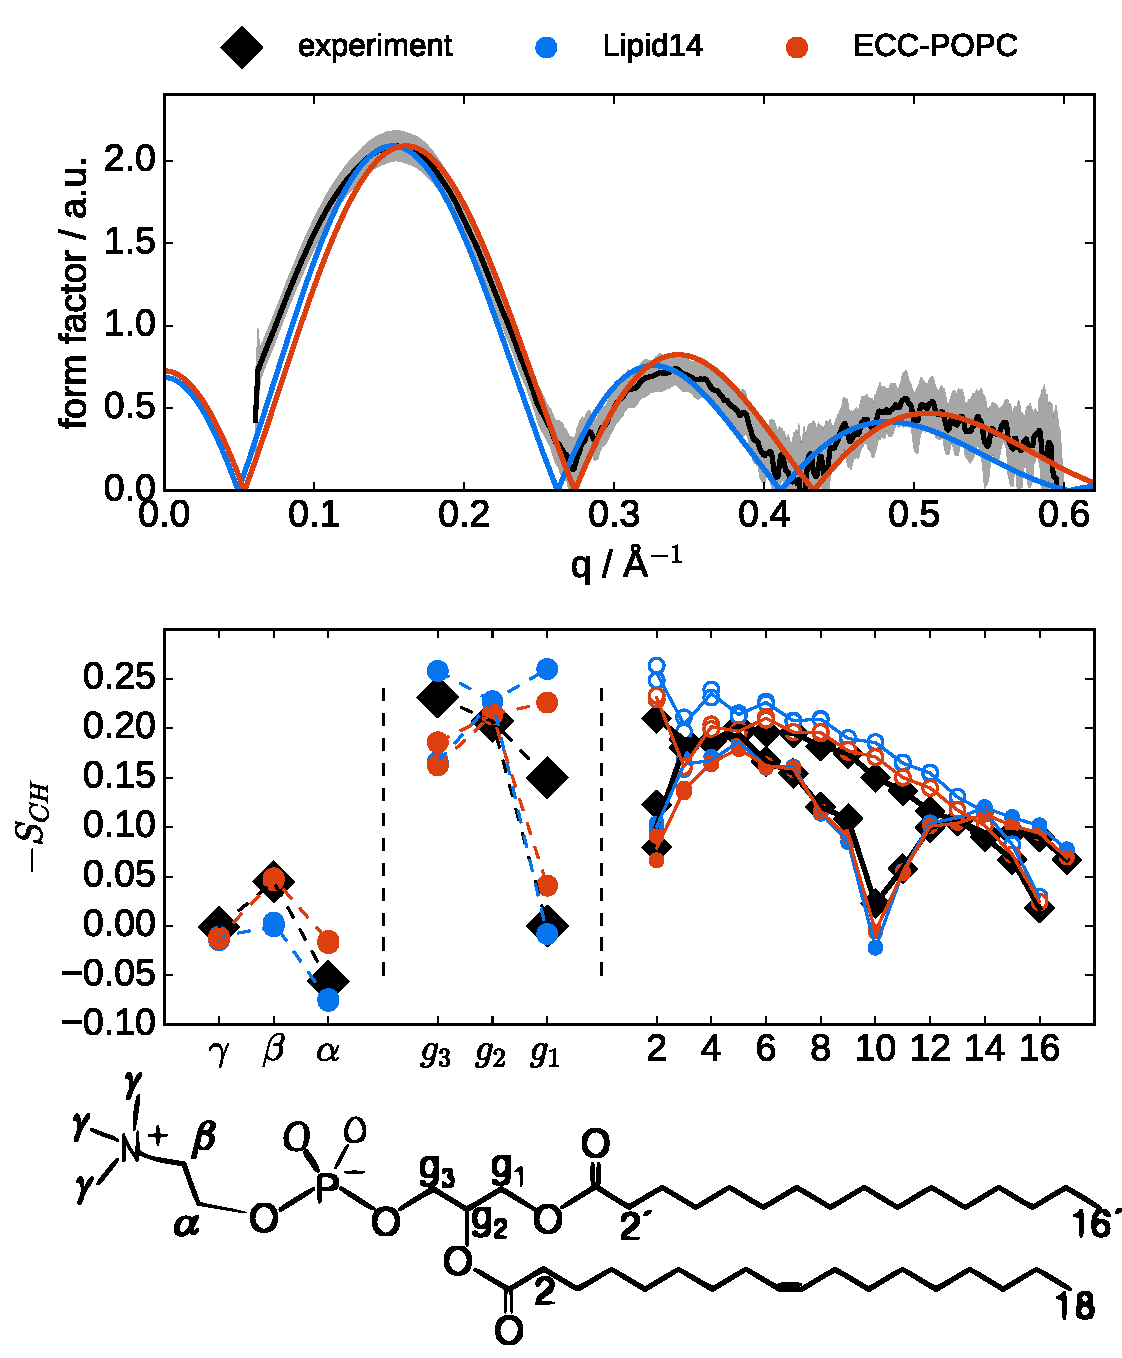
\includegraphics[width=8.2cm]{../img/ecc_pops/Order-parameters_form-factors_exp-L14-ECCL17_q80_sig89_POPC-struct.pdf} 
%  \caption{ \label{simVSexpNOions} 
%    Top: X-ray scattering form factors from simulations with the Lipid14 \citep{dickson14} and 
%    the ECC-POPC models compared with experiments~\citep{kucerka11} at 303~K. \\
%    Middle: Order parameters of POPC head group, glycerol backbone and acyl chains  
%    from simulations with the Lipid14 \citep{dickson14} and the ECC-POPC models 
%    compared with experiments \citep{ferreira13} at 300~K. 
%    The size of the markers for the head group order parameters correspond to 
%    the error estimate $\pm 0.02$ for experiments \citep{botan15,ollila16}, 
%    while the error estimate for simulations is $\pm 0.005$
%    (Bayesian estimate of 95\% confidence interval \citep{scipy}).
%    The size of the points for acyl chains are decreased by a factor of 3 to improve the clarity of the plot.
%    Open/closed symbols are used for palmitoyl/oleoyl chains of POPC. \\
%    Bottom: The chemical structure of POPC and the labeling of the carbon segments. 
%  }  
%\end{figure} 
 
\begin{table}[tb!] 
  \caption{Values of the area per lipid (APL) of POPC bilayers without ions. \label{tab:apls} 
  } 
  \begin{tabular}{l|c c} 
    model          & APL (Å$^2$)   & Temperature [K] \\ 
    \hline 
    Lipid14                   & 65.1$\pm$ 0.6  &  300 \\ 
    Lipid14 \citep{dickson14}  & 65.6$\pm$ 0.5  &  303 \\ 
    \hline 
    ECC-POPC                & 63.2$\pm$ 0.6  &  300       \\ 
    \hline 
    experiment \citep{kucerka11} & 64.3  &  303    \\ 
    \hline 
  \end{tabular} 
\end{table} 
 
 
First, we present results for bilayers in pure water. 
The ECC-POPC and Lipid14 models both reproduce the experimental X-ray scattering form factors 
of a POPC bilayer with a comparable accuracy (see Fig.~\ref{simVSexpNOions}). 
The area per lipid from the Lipid14 model is by $\approx$1Å larger than the 
experimental value in Table~\ref{tab:apls}, while the value from the ECC-POPC model 
is by $\approx$1Å smaller than the experimental one. 
The values of the area per lipid of the ECC-POPC model vary slightly 
when simulated with different water models (i.e., within the interval of 62.2--66.8 Å, see Table~S2 in SI), 
while still being close to the experimentally reported values. 
We can thus conclude that the ECC-POPC model reproduces the experimental dimensions of the POPC 
lipid bilayer with a comparable accuracy to other state-of-the-art lipid models~\citep{ollila16}. 
 
 
Similarly, the acyl chain order parameters of the ECC-POPC model, as well as those of the Lipid14 model~\citep{dickson14}, agree with the experimental values within the error bars, as presented in Fig.~\ref{simVSexpNOions}. Notably, the experimentally measured forking and small order parameter values of the $C_2$ segment in {\it sn}-2 chain are well reproduced by both models. This feature has been suggested to indicate that the carbonyl of the {\it sn}-2 chain is directed towards the water phase, in contrast to the carbonyl in the {\it sn}-1 chain, which orients more along the bilayer plane~\citep{seelig75,schindler75,gawrisch92}. 
This arrangement, which is not fully reproduced by other available lipid models~\citep{ollila16}, may be a relevant feature for the ion binding details. 
 
The order parameters of the $\alpha$ and $\beta$ carbons in the head group are slightly larger in the ECC-POPC model than in the Lipid14 model, which is apparently related to the P-N vector orienting by about 7$^{\circ}$ more toward the water phase in the former model, see Fig.~\ref{OrderParameterCHANGESsurf}. While both models perform relatively well, considering the available experimental evidence, it is not possible to decide which of the two models provides more realistic head group orientations. The ECC-POPC model gives the $\beta$ carbon order parameter value closer to experiments than the Lipid14 model, while the opposite is true for the $\alpha$ carbon. The accuracy of both models in the glycerol backbone region is comparable to other state-of-the-art lipid model available in literature \citep{botan15}, see Fig.~\ref{simVSexpNOions}. 


 
 
